\documentclass{article}

% If you need natbib options, place \PassOptionsToPackage before neurips_2026.
\usepackage{neurips_2026}

\usepackage[utf8]{inputenc}
\usepackage[T1]{fontenc}
\usepackage{hyperref}
\usepackage{url}
\usepackage{booktabs}
\usepackage{amsfonts}
\usepackage{microtype}
\usepackage{xcolor}
\usepackage{graphicx}
\usepackage{amsmath}
\usepackage{amssymb}
\usepackage{mathtools}
\usepackage{multirow}
\usepackage{pifont}

\graphicspath{{./}}

\newcommand{\cmark}{\ding{51}}
\newcommand{\xmark}{\ding{55}}

\title{HGWM: Hierarchical Graph-guided World Model for Zero-shot Object Navigation via Graph Matching}

% The submission version is anonymous by default in neurips_2026.
\author{Anonymous Author(s)}

\begin{document}

\maketitle

\begin{abstract}
Zero-shot object navigation requires agents to act under severe partial observability, where efficient search depends not only on recognizing visible semantics but also on anticipating unseen structure. Existing vision-language agents are strong at local recognition yet weak at reasoning about where promising regions are likely to be and which observations are structurally plausible. We introduce HGWM (Hierarchical Graph-guided World Model), which frames navigation as online graph matching between an LLM-derived predictive prior and a persistent spatial-semantic graph memory built from observations. HGWM uses a coarse-to-fine graph matching mechanism: a coarse semantic stage ranks frontier directions using goal-conditioned visual cues, and a fine structural stage verifies those candidates against predicted room-anchor relations while pruning inconsistent scene interpretations. Across HM3D and MP3D, HGWM delivers consistently strong performance, reduces looping, and remains robust across different foundation model choices. These results suggest that explicit structural prediction and coarse-to-fine grounding provide a more effective basis for zero-shot navigation than purely reactive exploration.
\end{abstract}

\section{Introduction}

Humans navigate unfamiliar environments by maintaining internal models to \textit{predict} the unseen—inferring that a bedroom likely leads to a bathroom, or that a kitchen implies a nearby dining area. This capacity for hierarchical spatial-semantic prediction enables efficient exploration through probabilistic mental maps. Conversely, while recent zero-shot navigation agents excel at semantic recognition using Foundation Models~\citep{yin2025unigoal,nie2025wmnav}, they lack mechanisms to \textit{anticipate} environmental topology, often resulting in redundant exploration when visual cues are ambiguous.

The core challenge is to move from reactive perception to predictive reasoning. Current methods face a fundamental dilemma. Vision-Language Models (VLMs) provide powerful open-vocabulary understanding~\citep{majumdar2022zson,nie2025wmnav}, yet remain \textit{myopic} by excelling at what they see now while struggling with where to look next given prior expectations. This manifests in two failure modes: (1) \textit{Perceptual Noise:} VLMs misidentify objects due to visual ambiguity, causing misguided exploration. (2) \textit{Structural Blindness:} Agents lack commonsense spatial constraints to reject implausible interpretations, resulting in inefficient trajectories.

To bridge this gap, we propose HGWM, a framework framed as a graph matching problem. An LLM generates an \textit{LLM-derived Predictive Prior} (Goal Subgraph) before observation. As the agent moves, a \textit{Spatial-Semantic Graph Memory} (Scene Graph) maintains physically grounded structure. HGWM then grounds predicted topology against perceived reality through a coarse-to-fine graph matching process: a coarse semantic stage quickly ranks frontier directions, while a fine structural stage verifies consistency and prunes noisy visual interpretations.

Our contributions are threefold:
\begin{itemize}
    \item We introduce HGWM, a navigation framework that converts goal semantics into a hierarchical predictive prior and grounds it online through a persistent spatial-semantic graph memory.
    \item We propose a coarse-to-fine graph matching mechanism that combines efficient semantic frontier ranking with fine structural verification for robust decision making under partial observability.
    \item We show on HM3D and MP3D that this design improves navigation efficiency and reduces looping, while component analysis highlights the roles of persistent memory and coarse-to-fine decision making.
\end{itemize}

We demonstrate HGWM's effectiveness on HM3D and MP3D, achieving 62.6\% SR on HM3D v0.1 (+4.5\% over WMNav) and 46.8\% on MP3D (+1.4\% over WMNav). Beyond raw success rates, HGWM significantly reduces repetitive exploration (looping) and exhibits high fault tolerance against severe visual ambiguity. Our component analysis further shows that persistent memory improves path efficiency, while the proposed coarse-to-fine matching contributes additional success-rate gains by filtering structurally implausible decisions. This supports the claim that structural prediction and coarse-to-fine grounding provide benefits beyond passive exploration alone.


\begin{figure*}[t]
\centering
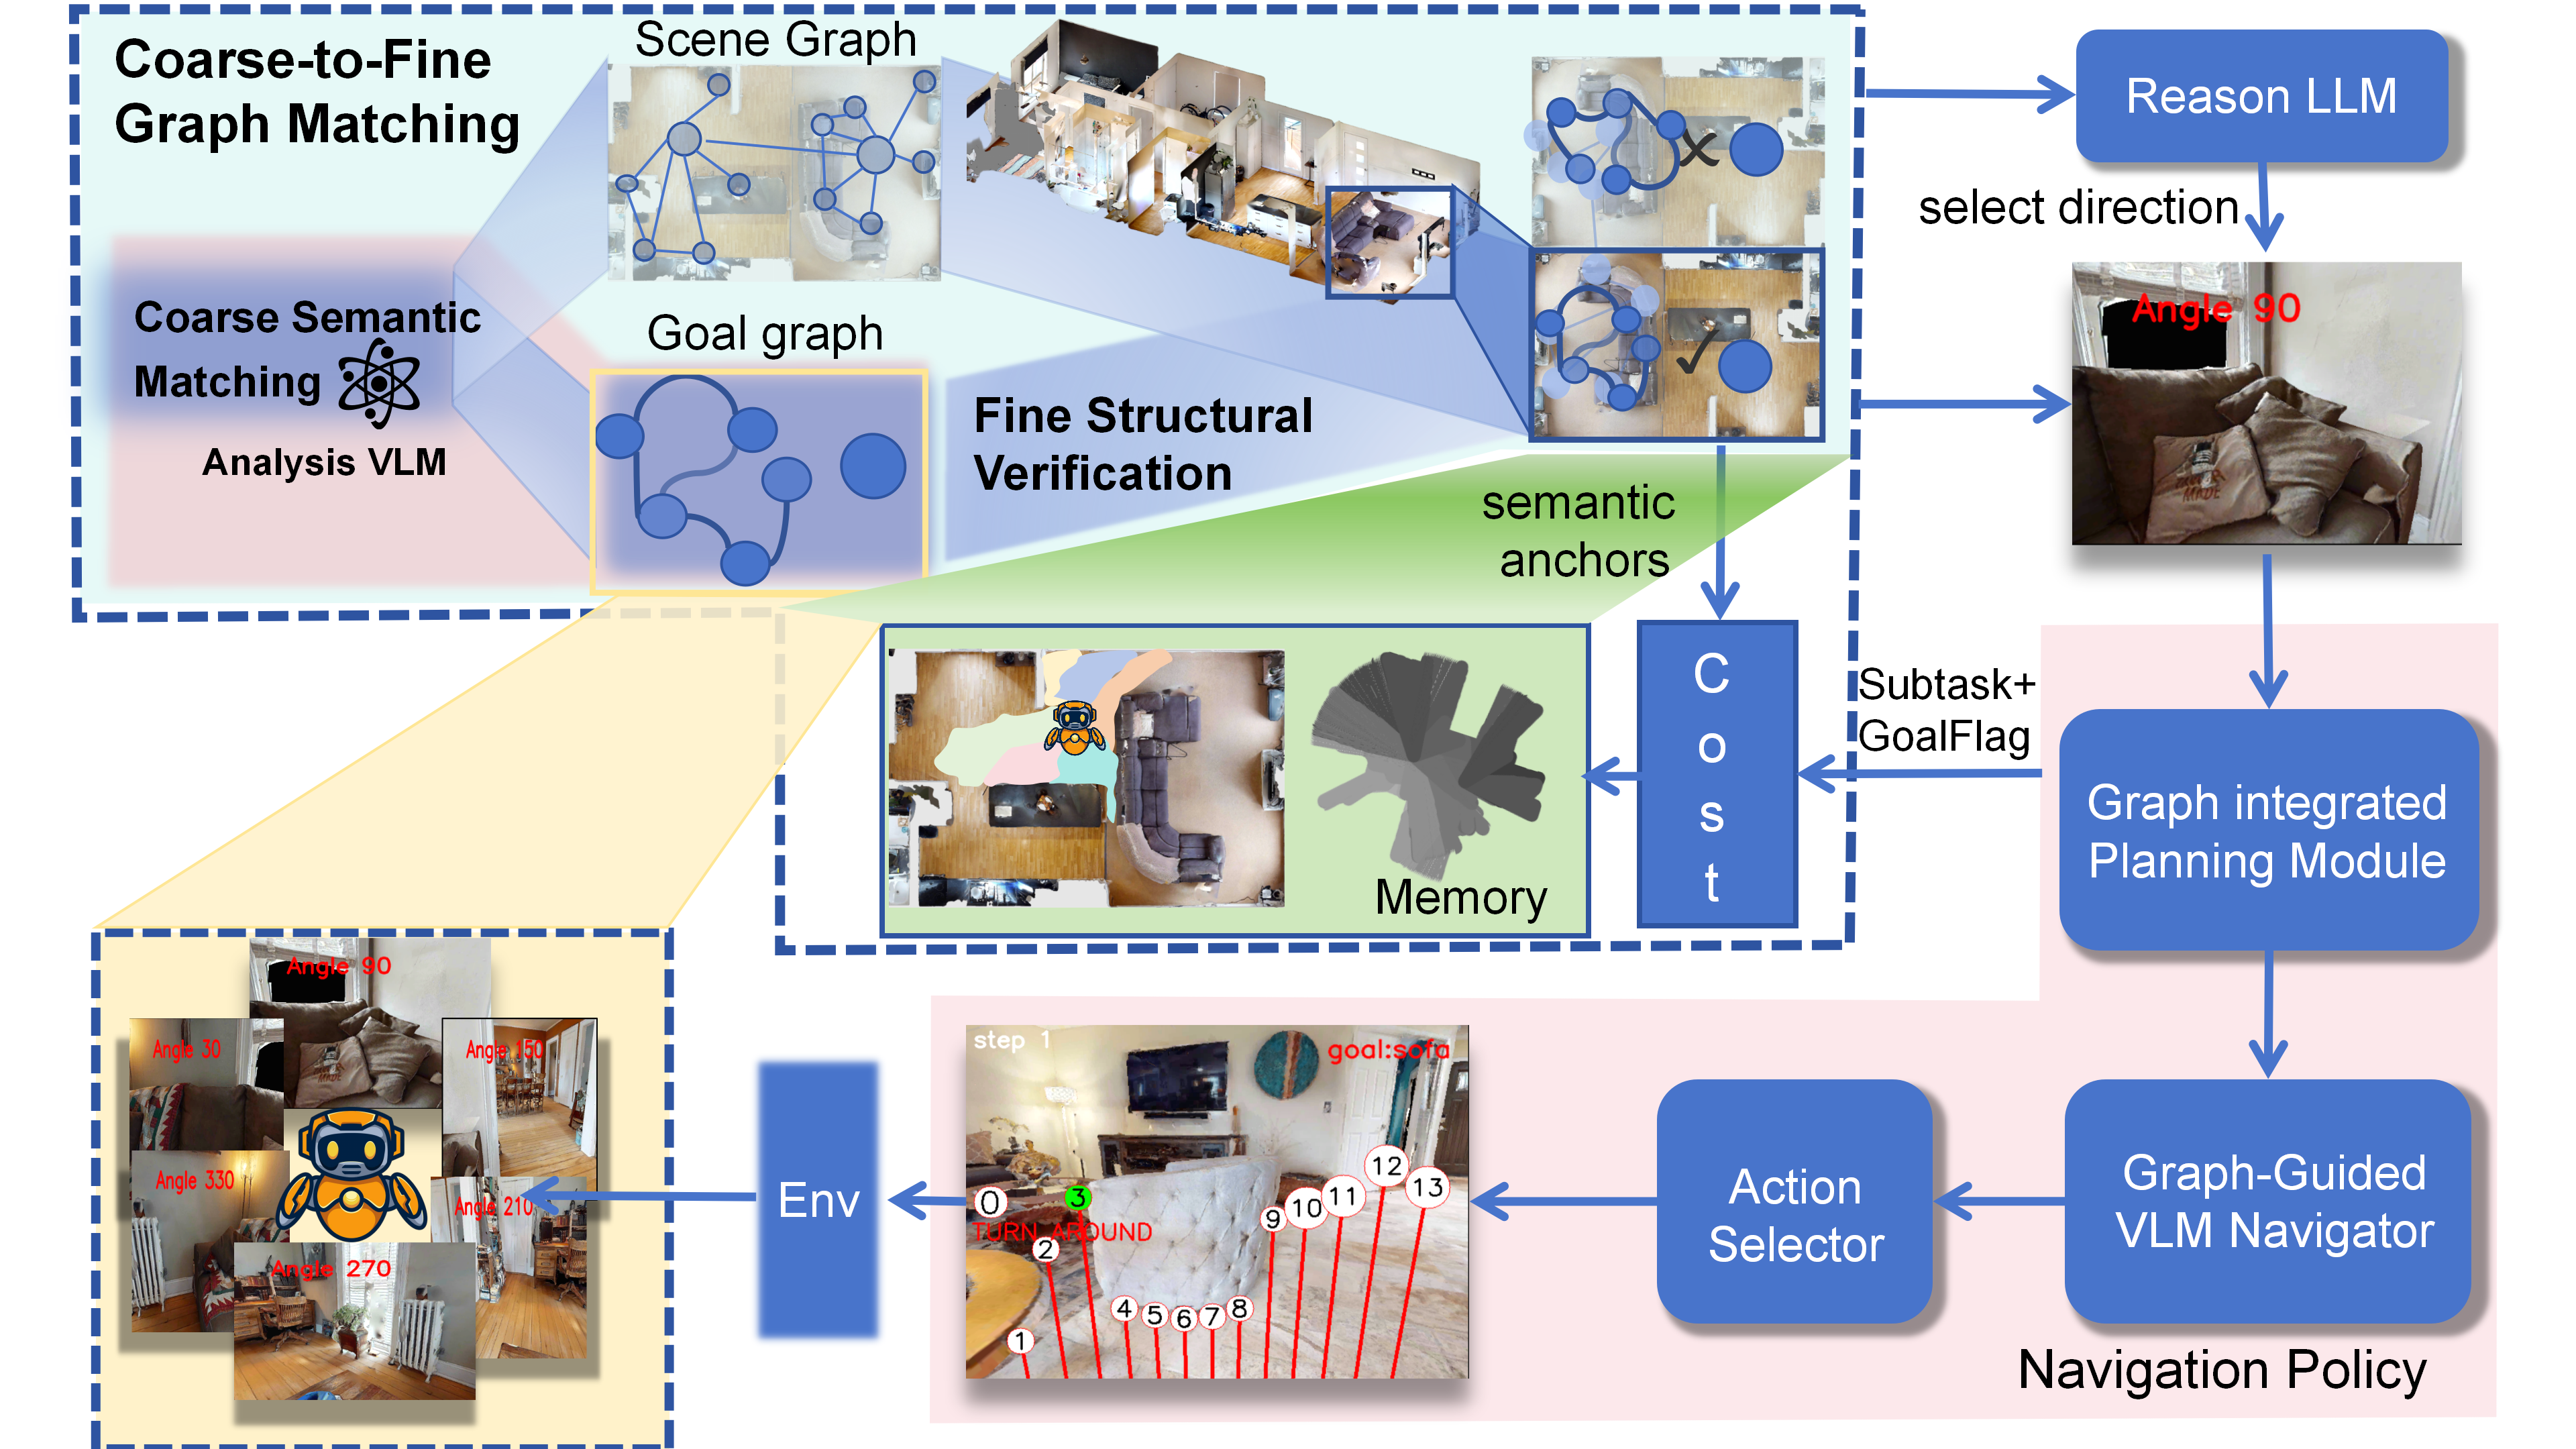
\includegraphics[width=1.0\textwidth]{architecture.png}
\caption{Overview of HGWM. The framework follows a \textit{Predict-Perceive-Ground} cycle: the LLM first hallucinates a predictive topological prior, the agent then grounds it against a persistent graph memory through online observations, and a cognitive arbitrator outputs the final navigation action.}
\label{fig:architecture}
\vspace{-0.4cm}
\end{figure*}

\section{Related Work}

Zero-shot object goal navigation. Recent surveys summarize the rapid progress of ObjectNav and multimodal navigation systems~\citep{sun2024survey,ieong2025multimodal}. Existing object navigation methods fall into two paradigms: supervised methods and zero-shot methods. Supervised approaches~\citep{ramrakhya2022habitat,yadav2023ovrl} lack generalizability. Zero-shot works~\citep{majumdar2022zson,gadre2023cows,zhou2023esc,kuang2024openfmnav,chen2023not} utilize foundation models for open-vocabulary understanding but typically treat navigation as reactive matching without persistent structural prediction. Recent advances such as 3D-Aware~\citep{zhang20233d}, ApexNav~\citep{zhang2025apexnav}, and BeliefMapNav~\citep{zhou2025beliefmapnav} improve frontier exploration and spatial representations, yet they still do not model unseen topology through an explicit predictive prior.

Graph-based scene representations.
While methods like SOON~\citep{zhu2021soon}, HOZ~\citep{zhang2021hierarchical}, and SG-Nav~\citep{yin2024sg} utilize graph or graph-like scene structures, they often rely on static or purely observed representations. ConceptGraphs~\citep{gu2024conceptgraphs} is particularly relevant because it incrementally builds an open-vocabulary 3D scene graph from observations. HGWM differs in two respects: it couples this observed graph memory with an LLM-derived predictive prior over unobserved structure, and it uses online graph matching between the prior and the observed graph to guide action selection. Closest to our work is UniGoal~\citep{yin2025unigoal}, which also aligns scene and goal graphs, but HGWM emphasizes a \textit{predict-then-ground} loop rather than an \textit{observe-then-map} pipeline.

World models and predictive representations.
Our approach builds on the world model paradigm~\citep{logue2018world,hafner2023mastering,koh2021pathdreamer}, which trains agents to learn latent dynamics models for planning. While these works focus on learning visual dynamics, we leverage foundation models to hallucinate symbolic topological priors~\citep{bar2025navigation}. This connects to predictive coding theories in neuroscience~\citep{friston2010free,clark2013whatever}, where the brain maintains generative models that are continuously updated via prediction errors.

Foundation model guided navigation. Recent advances highlight the complementary roles of VLMs and LLMs~\citep{nie2025wmnav}. However, current strong baselines often lack systematic integration of zero-shot foundation model capabilities with structured spatial reasoning and persistent graph memory, which HGWM addresses by establishing a consistency-check mechanism between a predictive prior and an observed graph memory.

\section{The Proposed Method}

We fundamentally reframe zero-shot object navigation: rather than treating it as a \textit{reactive search} task in a black-box environment, we define it as a graph matching problem. The core intuition is that efficient exploration stems from measuring the alignment between an agent's \textit{predicted} environmental topology (Predictive Prior $G_{goal}$) and its \textit{observed} structural memory (Grounded Graph Memory $G_{scene}^{(t)}$). Critically, this is not a static template-matching problem but a dynamic grounding process. At each timestep $t$, the agent's observation either strengthens or refutes hypotheses encoded in $G_{goal}$, progressively grounding the spatial structure.

To operationalize this idea, we introduce \textbf{HGWM} (Hierarchical Graph-guided World Model). Here, \textit{world model} refers to the joint predictive navigation state formed by the predictive prior, the observed graph memory, and their evolving alignment. As illustrated in Figure~\ref{fig:architecture}, HGWM first generates a probabilistic connectivity graph of the unseen environment via an LLM, and then actively grounds this prior against a persistent 3D spatial-semantic graph memory built from observations. Navigation decisions are therefore derived not merely from visual feature matching, but from continuously computing the structural graph matching score between $G_{goal}$ and $G_{scene}^{(t)}$.

\subsection{Problem Formulation}

We model the navigation task as a Partially Observable Markov Decision Process (POMDP) augmented with a structured spatial memory state. Let the target object category be $c$ (e.g., ``bed''). At each time step $t$, the agent receives an observation $O_t = \{I_t, D_t\}$ containing RGB and depth information, alongside its pose $P_t \in SE(2)$.

Unlike standard formulations that rely solely on a history vector, we define the agent's internal state as a \textit{Topological World Model} $\mathcal{W}_t = (G_{goal}, G_{scene}^{(t)}, \Psi_t)$, where $\Psi_t$ represents the matching distribution over possible topological paths. The key distinction is that the \textit{world model} denotes the full predictive state, whereas $G_{scene}^{(t)}$ itself is an observed graph memory built from sensor data. This predictive state is initialized with a generative prior $G_{goal} \sim P_{\text{LLM}}(\cdot|c)$ and a uniform match prior $\Psi_0$. At each step, physical observations drive proactive structural pruning:
\begin{equation}
\Psi_{t+1} \propto \Psi_t \cdot P(O_t | G_{scene}^{(t)}, G_{goal}),
\end{equation}
where structurally inconsistent observations receive near-zero probability, effectively pruning sensory noise from the semantic graph. The objective is to learn a policy $\pi(a_t | \mathcal{W}_t, O_t)$ that maximizes the likelihood of \textit{grounding} the abstract target node $v_{target} \in G_{goal}$ to a physical coordinate $p \in \mathbb{R}^3$ in minimal time. Success is defined as stopping when the agent's location is within a distance $d_{thres}$ of any instance of $c$, effectively verifying the complete alignment of the prediction to reality.

\begin{figure*}[ht]
\centering
\includegraphics[width=1.0\linewidth]{coarse_to_fine_matching.png}
\caption{Coarse-to-fine matching in HGWM. The coarse stage uses VLM-guided cues to rank frontier directions quickly, while the fine stage performs structural verification and proactive pruning to reject implausible scene interpretations before final action selection.}
\label{fig:coarse_to_fine}
\vspace{-0.2cm}
\end{figure*}

\subsection{LLM-Derived Predictive Prior}
\label{sec:goal_hallucination}
Unlike standard approaches that treat the goal as a mere semantic label (e.g., find a bed), we leverage the commonsense reasoning of LLMs to generate an LLM-derived predictive prior (visualized as the blue graph structure in Figure~\ref{fig:architecture}). This graph represents the agent's structural expectation of the unseen environment before exploration begins.
We denote this prior by $G_{goal} = \text{LLM}_{\text{hallucinate}}(\text{Goal}, \text{Prior Knowledge})$. As shown in the architecture, this prior is not a flat list but a hierarchical belief state comprising:
\begin{itemize}
    \item Room hypotheses (coarse nodes): probabilistic expectations of room types (e.g., Bedroom or Corridor) that act as containers for the target.
    \item Anchor cues (fine nodes): expected visual landmarks (e.g., Nightstand, Doorframe) that usually govern the connectivity to the target.
    \item Connectivity priors (edges): hallucinated transition probabilities between zones.
\end{itemize}
This structured hallucination provides the template against which physical observations are continuously verified, transforming navigation from a blind search into a structured grounding process.

\subsection{Spatial-Semantic Graph Memory as Physical Ground Truth}
\label{sec:world_model}

A fundamental innovation in HGWM is our Spatial-Semantic Graph Memory ($M_{world}$), which serves as the \textit{perceived reality} that anchors the hallucinated prior. Unlike the predictive topology $G_{goal}$, this memory is constructed only from actual observations and stores the physically grounded state of the environment.

For each panoramic observation, objects detected by the VLM are projected into the world coordinate system through depth-based mapping. We compute $P(o_i) = \text{Project}(o_i, D_t, P_t)$, where $o_i$ represents a detected object, $D_t$ provides depth information, and $P_t$ denotes the agent's current pose. The graph memory is then dynamically updated as $M_{world}[\text{key}(P(o_i))] \leftarrow \{o_i, \text{type}(o_i), \text{room}(o_i), \text{conf}(o_i)\}$, where $\text{key}(P(o_i))$ generates a unique spatial identifier for the object's 3D location. This integrated mapping system enables persistent spatial reasoning about objects and environments, even when they are no longer in the agent's immediate field of view, forming the foundation for dynamic scene graph construction and long-term spatial memory.

From this persistent memory, we dynamically construct direction-specific scene graphs $G_{scene}^{\alpha} = \text{GraphBuild}(M_{world}, \alpha)$ for each exploration direction $\alpha$ (a discrete heading increment radiating from the agent's current position toward unexplored regions). Each $G_{scene}^{\alpha}$ contains (i) \textit{Object Nodes} with spatial categorization, (ii) \textit{Room Classifications} with confidence scores, and (iii) \textit{Spatial Relationship Edges} encoding positional compatibility. This hierarchical representation provides the structured foundation for our topological grounding mechanism.

\subsection{Coarse-to-Fine Graph Matching Mechanism}
\label{sec:grounding}

The core engine of HGWM is a coarse-to-fine graph matching mechanism that continuously aligns the LLM-derived predictive prior $G_{goal}$ with the dynamic scene graph $G_{scene}^{\alpha}$. Rather than treating all candidate directions equally, HGWM first performs a coarse semantic screening and then applies fine-grained structural verification.

At initialization, the agent maintains a probabilistic expectation over the environment's topology encoded in $G_{goal}$ (e.g., Bedroom likely connects to Bathroom via Nightstand). As the agent explores, visual observations either confirm or contradict these expectations. The matching process therefore follows a coarse-to-fine design: a coarse semantic stage prioritizes frontier directions that appear semantically promising, and a fine structural stage validates whether those observations remain structurally consistent with the predictive prior before they influence downstream decisions.

This design is motivated by the asymmetric reliability of evidence across the episode. Early in exploration, the observed scene graph is sparse and incomplete, so aggressive structural verification can suppress promising frontiers simply because the agent has not yet seen enough context. In contrast, coarse semantic cues are cheap and useful for broad coverage at this stage. As more rooms, anchors, and transitions are accumulated, structural evidence becomes increasingly trustworthy, allowing the fine stage to reject visually plausible but topologically inconsistent hypotheses. HGWM therefore uses coarse semantic scoring to maintain exploration efficiency and fine structural verification to improve precision once sufficient context has been grounded.

Coarse semantic stage. The VLM provides a direct heuristic assessment of the visual field via $S_{\text{coarse}}(\alpha) = \text{VLM}(I_{\text{panoramic}}, \text{Prompt}(G_{goal}))$, where the prompt is enriched with target room types, anchor objects, and spatial context. In practice, the VLM is prompted to return a scalar plausibility score for each direction on a fixed 1--9 scale, and these textual scores are linearly normalized within the candidate set before ranking. This stage efficiently ranks candidate directions using immediate visual semantics and is especially useful during frontier exploration. However, raw VLM outputs are noisy and prone to hallucinations, so coarse ranking alone is insufficient for reliable navigation.


\begin{figure}[t]
\centering
\includegraphics[width=0.7\linewidth,trim=18 12 18 12,clip]{graph_matching_pipeline.png}
\caption{Fine structural matching pipeline. The LLM first prunes structurally implausible nodes from the raw scene graph, then the corrected graph is embedded and matched against the predictive prior.}
\label{fig:graph_matching_pipeline}
\vspace{-0.5cm}
\end{figure}

Fine structural stage. To correct potential VLM noise and perform robust structural verification, we employ a multi-stage approach (Figure~\ref{fig:graph_matching_pipeline}).

\textit{Stage 2.1: Proactive Structural Pruning.} 
Before matching, the LLM analyzes the local observation $G_{scene}^{\alpha}$ against the predictive prior $G_{goal}$. Because navigation views are often blurred, truncated, or out-of-context, the system applies structural constraints to discard noisy perceptual errors. If the observation contains implausible patterns (e.g., Toilet detected in Kitchen), the system proactively prunes the corresponding nodes/edges, yielding $G_{corrected}^{\alpha} = \text{LLM}_{\text{prune}}(G_{scene}^{\alpha}, G_{goal})$. This step prevents sensory noise from propagating into downstream decisions.

\textit{Stage 2.2: Multi-dimensional Graph Embedding.} 
After filtering observational noise, we compute a structural similarity score $S_{\text{fine}}(\alpha) = (w_{obj} S_{obj} + w_{room} S_{room} + w_{spatial} S_{spatial}) \cdot D(\alpha) \cdot R(\alpha)$ by embedding nodes into a shared semantic space and performing weighted graph matching. Here, $S_{obj}$ represents the semantic similarity between observed objects and goal-associated objects, $S_{room}$ measures the alignment of the currently inferred room type with the target room hypothesis, and $S_{spatial}$ evaluates the consistency of spatial layouts against the goal graph. We utilize fixed, interpretable weights ($w_{obj}=0.4, w_{room}=0.3, w_{spatial}=0.2$), prioritizing object presence and room context. $D(\alpha)$ is a directional factor (1.0 for forward, decaying backward) and $R(\alpha)$ represents the fraction of matched goal anchors.

To further stabilize this stage, we apply a position-aware enhancement $S_{\text{fine}}'(\alpha) = S_{\text{fine}}(\alpha)\cdot \text{PositionScore}(\alpha)$, where the position factor favors forward-facing candidates, rewards geometrically consistent object layouts, and boosts doorway or hallway transitions that lead toward predicted room types. This fine structural score serves as a filter for the coarse semantic signal, ensuring that navigation decisions respect the spatial organization of the graph memory.

\subsection{Cognitive Fusion and Navigation Policy}

The final navigation decision fuses the coarse semantic signal and the fine structural signal through an LLM-based arbitrator. Based on the overlap between $G_{goal}$ and $G_{scene}$, HGWM implements an adaptive three-stage policy: \textit{Frontier Exploration} (overlap $< 0.3$), \textit{Focused Search} ($0.3 \leq \text{overlap} < 0.7$), and \textit{Target Verification} (overlap $\geq 0.7$). This schedule naturally mirrors the coarse-to-fine progression of the method: early exploration favors broad semantic coverage, while later stages rely increasingly on structural verification for precise localization.

The two signals are complementary rather than redundant: the coarse score captures immediate visual-semantic promise (e.g., does this direction look like it leads to a bedroom?), whereas the fine score tests structural plausibility against the predicted topology (e.g., is this local scene arrangement compatible with the target room and its anchors?). Accordingly, HGWM emphasizes spatial coverage during frontier exploration with $(w_{\text{spatial}}, w_{\text{llm}})=(0.7, 0.3)$, balances both signals during focused search with $(0.5, 0.5)$, and prioritizes precise verification during target localization with $(0.3, 0.7)$.

The LLM reasoning component synthesizes all available information as $S_{\text{llm}}(\alpha) = \text{LLM}_{\text{integrate}}(G_{scene}^{\alpha,(t+1)}, S_{\text{coarse}}(\alpha), S_{\text{fine}}'(\alpha), G_{\text{goal}}, \text{Phase})$. Here the LLM receives the normalized coarse and fine scores, the current phase, and the local scene graph, and returns a textual scalar confidence that is parsed into $S_{\text{llm}}(\alpha)$. We then combine it with a distance-based heuristic using $\text{Score}_{\text{final}}(\alpha) = w_{\text{spatial}} \cdot S_{\text{base}}(\alpha) + w_{\text{llm}} \cdot S_{\text{llm}}(\alpha)$, where $S_{\text{base}}(\alpha)$ favors navigable free space based on depth geometry.

This fusion is designed to avoid double-counting rather than simply averaging two correlated scores. The coarse stage acts as a high-recall selector that rapidly proposes visually promising directions, while the fine stage serves as a structural filter that suppresses locally plausible but topologically inconsistent candidates. In practice, both scores are normalized within the candidate set before arbitration, allowing the LLM to compare their relative confidence under the current exploration phase rather than their raw magnitudes. As a result, the fused policy behaves conservatively when structural evidence is weak and becomes progressively more verification-driven once enough graph context has been accumulated.

\begin{table*}[ht]
\caption{Comparison with representative object navigation methods on HM3D v0.1 and MP3D benchmarks. US denotes Unsupervised capabilities (e.g., relying on no pre-explored maps or specific geometric assumptions, thus VLFM is marked \xmark\ as it relies on calibrated geometric map assumptions), ZS denotes Zero-Shot capabilities, and II denotes Instruction Interpolator.}
\label{tab:main_results}
\centering
\small
	\resizebox{1\linewidth}{!}{% 
\begin{tabular}{l|c|c|l|l|cc|cc}
\hline
\multirow{2}{*}{\textbf{Method}} & \multirow{2}{*}{\textbf{US}} & \multirow{2}{*}{\textbf{ZS}} & \multirow{2}{*}{\textbf{Vision}} & \multirow{2}{*}{\textbf{Language}} & \multicolumn{2}{c|}{\textbf{HM3D v0.1}} & \multicolumn{2}{c}{\textbf{MP3D}} \\
& & & & & \textbf{SR↑} & \textbf{SPL↑} & \textbf{SR↑} & \textbf{SPL↑} \\
\hline
Habitat-Web~\citep{ramrakhya2022habitat} & \xmark & \xmark & - & - & 41.5 & 16.0 & 31.6 & 8.5 \\
OVRL~\citep{yadav2023ovrl} & \xmark & \xmark & - & - & - & - & 28.6 & 7.4 \\
OVRL-V2~\citep{yadav2023ovrl} & \xmark & \xmark & - & - & 64.7 & 28.1 & - & - \\
ZSON~\citep{majumdar2022zson} & \xmark & \cmark & CLIP & - & 25.5 & 12.6 & 15.3 & 4.8 \\
PSL~\citep{sun2024prioritized} & \xmark & \cmark & CLIP & - & 42.4 & 19.2 & 18.9 & 6.4 \\
PixNav~\citep{cai2024bridging} & \xmark & \cmark & LLaMA-Adapter & GPT-4 & 37.9 & 20.5 & - & - \\
SGM~\citep{zhang2021hierarchical} & \xmark & \cmark & - & - & 60.2 & 30.8 & 37.7 & 14.7 \\
VLFM~\citep{yokoyama2024vlfm} & \xmark & \cmark & BLIP-2 & - & 52.5 & 30.4 & 36.4 & 17.5 \\
\hline
CoW~\citep{gadre2023cows} & \cmark & \cmark & CLIP & - & - & - & 9.2 & 4.9 \\
ESC~\citep{zhou2023esc} & \cmark & \cmark & - & GPT-3.5 & 39.2 & 22.3 & 28.7 & 14.2 \\
L3MVN~\citep{yu2023l3mvn} & \cmark & \cmark & - & GPT-2 & 50.4 & 23.1 & - & - \\
VoroNav~\citep{wu2024voronav} & \cmark & \cmark & BLIP & GPT-3.5 & 42.0 & 26.0 & - & - \\
HyPerNav~\citep{yin2025hypernav} & \cmark & \cmark & Qwen-VL-7B-Instruct & - & 56.3 & 29.7 & 43.8 & 16.9 \\
TopV-Nav~\citep{zhong2024topv} & \cmark & \cmark & - & - & 45.9 & 28.0 & 31.9 & 16.1 \\
SG-Nav~\citep{yin2024sg} & \cmark & \cmark & LLaVA-1.6-7B & GPT-4 & 54.0 & 24.9 & 40.2 & 16.0 \\
UniGoal~\citep{yin2025unigoal} & \cmark & \cmark & LLaVA-1.6-7B & LLaMA-2-7B & 54.5 & 25.1 & 41.0 & 16.4 \\
WMNav~\citep{nie2025wmnav} & \cmark & \cmark & Gemini-1.5-Pro & - & 58.1 & 31.2 & 45.4 & 17.2 \\
\hline
\textbf{HGWM (Ours)} & \cmark & \cmark & \textbf{Gemini-1.5-Pro} & \textbf{Qwen2.5-7B-Instruct} & \textbf{62.6} & \textbf{31.5} & \textbf{46.8} & \textbf{17.9} \\
\hline
\end{tabular}}
\vspace{-0.4cm}
\end{table*}

\subsection{Navigation Policy}

The policy layer in HGWM converts graph matching signals into executable navigation decisions. Instead of mapping local observations directly to actions, the agent maintains a graph-conditioned decision state that combines the current scene graph, the predictive goal prior, and the exploration phase. This state supports the generation of semantically meaningful subtasks that are aligned with long-horizon search, such as approaching a predicted room transition or validating a likely anchor region before final goal localization.

Operationally, HGWM uses graph-guided subtask decomposition, $\text{SubTask}_t, \text{GoalFlag}_t = \text{PlanVLM}(I_t(\alpha), \text{SubTask}_{t-1}, G_{scene}^{\alpha,(t)}, G_{goal})$, to translate structural context into short-horizon objectives. Candidate actions $A_t^{cand} = \{(r_{t,j}, \theta_{t,j})\}_{j=1}^{K'}$ are then re-ranked by the coarse-to-fine matching mechanism instead of local exploration heuristics alone. During frontier exploration, the coarse semantic stage favors directions that are visually consistent with likely target regions; during focused search and target verification, the fine structural stage increasingly favors candidates supported by room-anchor compatibility and spatial consistency. The final action is selected by reasoning over annotated observations and scene-graph context, $a_t = \text{ReasonVLM}(\text{SubTask}_t, \text{Goal}_t, I_t^{ann}, G_{scene}^{\alpha,(t)})$. In this sense, the policy operates as a graph-conditioned decision rule: coarse semantic cues preserve search efficiency, while fine structural validation suppresses locally plausible but globally inconsistent moves.



\section{Experiments}

We conduct comprehensive experiments on two standard benchmarks to evaluate HGWM for zero-shot object navigation. Our experimental design focuses on demonstrating the effectiveness of graph-guided reasoning in diverse indoor environments while maintaining unsupervised and zero-shot capabilities.


\subsection{Datasets and Evaluation Metrics}

Datasets. We evaluate on HM3D v0.1, HM3D v0.2, and MP3D~\citep{ramakrishnan2021habitat,chang2017matterport3d}. We report main comparisons on HM3D v0.1 for consistency with prior work, and use the cleaner HM3D v0.2 split for ablations that isolate graph matching and structural pruning effects.

Evaluation metrics. We report Success Rate (SR) and Success weighted by Path Length (SPL), following standard ObjectNav evaluation protocols~\citep{anderson2018evaluation,batra2020objectnav}. These metrics measure navigation effectiveness and efficiency, respectively. Figure~\ref{fig:comparison} provides qualitative evidence that HGWM reduces looping and encourages exploration toward more informative regions.

\subsection{Main Results}

HGWM performs strongly across both benchmarks (Table~\ref{tab:main_results}). On HM3D v0.1, it achieves 62.6\% SR and 31.5\% SPL, improving over WMNav~\citep{nie2025wmnav} by +4.5\% SR and +0.3\% SPL. On MP3D, it achieves 46.8\% SR and 17.9\% SPL, corresponding to gains of +1.4\% SR and +0.7\% SPL over WMNav.

Compared to learning-based methods such as OVRL-V2~\citep{yadav2023ovrl}, HGWM retains zero-shot generalization without task-specific training. Among zero-shot methods, it outperforms ZSON~\citep{majumdar2022zson}, VLFM~\citep{yokoyama2024vlfm}, and graph-based approaches such as SG-Nav~\citep{yin2024sg} and UniGoal~\citep{yin2025unigoal}, indicating that predictive structural grounding is effective for navigation in complex indoor scenes.

\begin{figure*}[t]
    \centering
    \includegraphics[width=0.98\linewidth]{Comparison.jpg}
    \caption{Decision process comparison between WMNav and HGWM. HGWM leverages graph-based memory to avoid repetitive exploration in the same space and encourages the agent to move toward regions with greater object visibility, resulting in more efficient and diverse exploration trajectories compared to WMNav.}
    \vspace{-0.2cm}
    \label{fig:comparison}
\end{figure*}

\subsection{Backbone Robustness}

To test backbone sensitivity, we evaluate HGWM with different VLMs on HM3D v0.1 in Table~\ref{tab:vlm_robustness}. The default Gemini-1.5-Pro setting achieves 62.6\% SR and 31.5\% SPL, while the lighter Gemini 2.0 Flash reaches 59.2\% SR and 30.8\% SPL. This modest drop suggests that the main gain comes from graph-guided memory and predictive-prior coupling rather than any single backbone.

Notably, the backbone change affects SR more than SPL. This pattern suggests that weaker VLM reasoning mainly degrades semantic recall and room-level recognition, while the geometric component of the policy remains comparatively stable once a plausible direction has been selected. In other words, the coarse-to-fine design does not remove backbone dependence, but it prevents moderate VLM degradation from collapsing the entire navigation pipeline.

\begin{table}[t]
\centering
\caption{Backbone robustness on HM3D v0.1. HGWM remains effective across different VLM backbones.}
\label{tab:vlm_robustness}
\footnotesize
\setlength{\tabcolsep}{4pt}
\begin{tabular}{l|cc|cc}
\hline
\multirow{2}{*}{\textbf{VLM Backbone}} & \multicolumn{2}{c|}{\textbf{HGWM}} & \multicolumn{2}{c}{\textbf{Relative Change}} \\
& \textbf{SR(\%)↑} & \textbf{SPL(\%)↑} & \textbf{SR} & \textbf{SPL} \\
\hline
Gemini-1.5-Pro (Default) & \textbf{62.6} & \textbf{31.5} & - & - \\
Gemini 2.0 Flash & 59.2 & 30.8 & -3.4\% & -0.7\% \\
\hline
\end{tabular}
\vspace{-0.2cm}
\end{table}

% ...existing code...

\subsection{Component Analysis}

We analyze the contribution of each HGWM component on HM3D v0.2~\citep{ramakrishnan2021habitat} in Table~\ref{tab:ablation_study}. Basic VLM navigation without memory achieves 67.8\% SR and 29.3\% SPL. Adding voxel memory improves performance to 70.9\% SR and 32.8\% SPL, indicating that persistent spatial storage is a major source of path-efficiency gains. Replacing this memory with hierarchical graph memory and coarse-to-fine matching further increases success to 74.4\% SR, yielding an additional +3.5 SR over the voxel-memory baseline while maintaining comparable path efficiency.

Sensitivity and behavioral robustness. The ablation trend suggests a clear division of labor. Voxel memory primarily shortens paths once useful observations have been accumulated, whereas hierarchical graph memory with coarse-to-fine matching improves the reliability of directional decisions under perceptual ambiguity. The slightly lower SPL of the full model suggests that fine structural verification may occasionally accept a small path-length cost in exchange for a larger improvement in success, which is consistent with the qualitative comparisons in Figure~\ref{fig:comparison}. Overall, these results support the intended design of HGWM: coarse semantic cues improve recall during exploration, while fine structural verification improves precision when the agent approaches goal-relevant regions.

This pattern is consistent with the intended role of each module. Direct VLM scoring is effective for recognizing immediately visible goal-related cues, but it cannot determine whether those cues are structurally compatible with the predicted room layout or anchor configuration. Voxel memory improves efficiency by preserving previously explored free space, yet it remains largely geometric and therefore cannot distinguish between semantically similar but topologically different regions. The hierarchical graph memory closes this gap by introducing explicit room-object-anchor relations, which is especially valuable in repeated layouts and ambiguous transitional spaces such as hallways, doorways, and partially observed rooms.


\begin{table}[t]
\centering
\caption{Component analysis on HM3D v0.2~\citep{ramakrishnan2021habitat}. Voxel memory improves path efficiency, while hierarchical graph memory with coarse-to-fine matching further improves success under ambiguity.}
\label{tab:ablation_study}
\resizebox{\linewidth}{!}{
\begin{tabular}{l|l|l|cc}
\hline
\textbf{Method} & \textbf{Memory Structure} & \textbf{Decision Signal} & \textbf{SR(\%)↑} & \textbf{SPL(\%)↑} \\
\hline
Basic VLM Nav & \xmark\ None & Direct VLM Scoring & 67.8 & 29.3 \\
VLM + Memory & \cmark\ Voxel Memory & Direct VLM Scoring & 70.9 & 32.8 \\
\textbf{HGWM (Ours)} & \cmark\ Hierarchical Graph Memory & Coarse-to-fine Matching & \textbf{74.4} & \textbf{31.9} \\
\hline
\end{tabular}
}
\vspace{-0.2cm}
\end{table}


\subsection{Efficiency and Limitations}

To assess the computational overhead introduced by large vision-language models, we measure the latency of a single navigation step. Using Gemini-1.5-Pro, one inference step requires approximately 2.3 seconds on average. Although this latency is higher than that of end-to-end trained policies, the resulting overhead can be partially hidden by overlapping API calls with physical robot motion in real deployments.

Importantly, this overhead is dominated by foundation-model inference rather than graph maintenance itself. In our implementation, graph updates require only lightweight spatial hashing and local matching operations, so the memory module adds negligible runtime compared with a single VLM call. We also pre-generate goal priors with deterministic prompts and reuse cached responses for repeated queries, which keeps evaluation reproducible and reduces unnecessary variance across runs.

This cost profile is favorable for asynchronous deployment. Graph memory can be updated online with minimal delay, while slower semantic modules can be queried less often or overlapped with robot motion. As a result, the main bottleneck is not maintaining structured state, but deciding how often high-capacity foundation models should be invoked.

HGWM also has several limitations that motivate future work: (1) \textit{Foundation Model Dependency and Compute:} performance remains constrained by the capabilities of the underlying VLMs, and low-power settings will likely require distilling structural reasoning into smaller local models; (2) \textit{Sim-to-Real Transfer:} the current evaluation is restricted to Habitat, while physical deployment introduces sensor noise and localization errors that may destabilize structural verification; and (3) \textit{Structured Environment Assumptions:} HGWM relies on common indoor topological regularities, and extending it to highly unstructured or outdoor settings remains an open problem.

\section{Conclusion}

We presented HGWM, a zero-shot navigation framework that matches an LLM-derived predictive prior against persistent graph memory through coarse-to-fine graph matching. Results on HM3D and MP3D show strong performance, stable behavior across backbones, and improved robustness in ambiguous episodes, suggesting that explicit structural prediction complements reactive foundation-model navigation in partially observed environments.

% \section{Discussion}
% TODO: Interpret results, discuss limitations, implications

% Acknowledgements should only appear in the accepted version.
% \section*{Acknowledgements}

% \textbf{Do not} include acknowledgements in the initial version of the paper
% submitted for blind review.

% If a paper is accepted, the final camera-ready version can (and usually should)
% include acknowledgements.  Such acknowledgements should be placed at the end of
% the section, in an unnumbered section that does not count towards the paper
% page limit. Typically, this will include thanks to reviewers who gave useful
% comments, to colleagues who contributed to the ideas, and to funding agencies
% and corporate sponsors that provided financial support.


\bibliography{neurips_2026_conference}
\bibliographystyle{plain}

%%%%%%%%%%%%%%%%%%%%%%%%%%%%%%%%%%%%%%%%%%%%%%%%%%%%%%%%%%%%%%%%%%%%%%%%%%%%%%%
% APPENDIX
%%%%%%%%%%%%%%%%%%%%%%%%%%%%%%%%%%%%%%%%%%%%%%%%%%%%%%%%%%%%%%%%%%%%%%%%%%%%%%%
\newpage
\appendix

\section{Goal Prior Construction}
\label{sec:goal_construction}

\subsection{LLM Prompt Template}

We present the complete prompt template used for goal subgraph construction. The template is dynamically instantiated for each target object category, with \texttt{\{goal\}} replaced by the specific target (e.g., ``bed'', ``sofa'').

\begin{quote}
\small
\texttt{You are an expert in residential navigation and spatial understanding. Create a comprehensive navigation strategy for efficiently locating a \{GOAL\} in a typical home environment.}

\texttt{NAVIGATION STRATEGY ANALYSIS FOR \{GOAL\}:}

\texttt{1. TARGET ROOM ANALYSIS:}\\
\texttt{~~(1) Primary room: The most likely room type where \{goal\} is typically found}\\
\texttt{~~(2) Secondary rooms: 1-2 alternative room types where \{goal\} might also be located}\\
\texttt{~~(3) Adjacent zones: Connected areas that provide visual access or pathways to target rooms}

\texttt{2. PATHWAY and CONNECTIVITY MAPPING:}\\
\texttt{~~(1) Hallway connections: Common routes to reach target rooms from main areas}\\
\texttt{~~(2) Visual access points: Doorways/openings that help identify target rooms}\\
\texttt{~~(3) Navigation landmarks: Key reference points for wayfinding}

\texttt{3. TARGET-ORIENTED SPATIAL ANCHORS and NAVIGATION CUES:}\\
\texttt{~~(1) Directional anchors: 3-4 objects that DIRECTLY indicate where \{goal\} is likely located}\\
\texttt{~~(2) Visual pathways: Objects that form visual lines leading toward typical \{goal\} placement areas}\\
\texttt{~~(3) Distance indicators: Objects that help estimate proximity to \{goal\}}\\
\texttt{~~(4) Positioning cues: Furniture/fixtures indicating the specific area where \{goal\} is usually found}

\texttt{4. SYSTEMATIC EXPLORATION APPROACH:}\\
\texttt{~~(1) Exploration priorities: Which areas to check first when searching}\\
\texttt{~~(2) Recovery strategies: What to do when initial search paths fail}
\end{quote}

This structured prompt enables the LLM to generate hierarchical spatial knowledge encompassing room classifications, connectivity patterns, and object-based navigation cues, which are then parsed into the formal goal subgraph representation $G_{goal} = (V_{goal}, E_{goal})$ where nodes represent rooms/objects and edges encode spatial relationships.

\section{Implementation Details}
\label{app:implementation}

\subsection{Agent Configuration}
We configure the agent with a maximum of 40 navigation steps per episode. The agent has a cylindrical body with radius 0.18m and height 0.88m, equipped with an egocentric RGB-D camera at 640×480 resolution and 79° horizontal FOV. The camera is tilted down with a 14° pitch to improve navigable area identification. The success threshold $d_{thres}$ is set to 1.0m. We primarily use Gemini-1.5-Pro VLM for experiments due to its cost-effectiveness and strong spatial reasoning capabilities.

\subsection{Model Choices}
\textbf{VLM Backbone:} Gemini-1.5-Pro serves as our primary vision-language model for both scene understanding (object detection, room classification) and coarse semantic scoring. We chose this model for its superior performance on spatial reasoning tasks and cost-efficiency compared to GPT-4V.

\textbf{LLM Reasoner:} Qwen2.5-7B-Instruct is used for graph construction, structural pruning, and decision arbitration. This open-source model provides strong commonsense reasoning while being deployable locally, eliminating API latency concerns.

\section{Coarse-to-Fine Reasoning}
\label{app:multistage}

\subsection{Stage Scheduling}

Our navigation system employs three distinct exploration phases, each optimized for different levels of goal-environment correspondence:

\textbf{Phase 1: Frontier Exploration.} Activated when overlap $< 0.3$ between $G_{goal}$ and $G_{scene}$, indicating limited environmental knowledge. The system prioritizes systematic exploration with weights heavily favoring spatial coverage ($w_{\text{spatial}}=0.7, w_{\text{llm}}=0.3$). The agent focuses on discovering new areas and building comprehensive environmental understanding through frontier-based exploration.

\textbf{Phase 2: Focused Search.} Engaged when $0.3 \leq \text{overlap} < 0.7$, suggesting goal-relevant environmental features are detected. This phase employs balanced weights ($w_{\text{spatial}}=0.5, w_{\text{llm}}=0.5$) to achieve optimal exploration-exploitation trade-offs. The system begins leveraging discovered anchor objects and spatial relationships for directed search.

\textbf{Phase 3: Target Verification.} Triggered when overlap $\geq 0.7$, indicating a high likelihood of goal proximity. This phase applies comprehensive LLM-based scene graph correction and prioritizes precise localization ($w_{\text{spatial}}=0.3, w_{\text{llm}}=0.7$). The agent concentrates on detailed verification and accurate goal identification through rigorous structural consistency checks.

\subsection{Position-Aware Scoring}

To address the limitation that standard semantic embeddings lack spatial awareness, we augment the fine structural score with position-aware factors using $S_{\text{enhanced}} = S_{\text{fine}}(\alpha) \cdot \text{PositionScore}(\alpha)$, where $\text{PositionScore}(\alpha)$ incorporates:
\begin{itemize}
    \item \textit{Directional Bias:} Forward-facing directions receive higher weights (1.0) while backward directions decay exponentially ($0.3-0.5$), reflecting natural exploration bias.
    \item \textit{Spatial Consistency:} Objects appearing in geometrically consistent configurations (e.g., ``bed near nightstand") receive bonus multipliers.
    \item \textit{Room Transition Cues:} Doorway/hallway detections boost scores for directions leading to unexplored room types predicted in $G_{goal}$.
\end{itemize}

\subsection{Reproducibility Details}

To ensure deterministic behavior and eliminate stochasticity from LLM generation during evaluation, we implement a strict caching strategy:

\textbf{Goal Graph Caching.} We pre-generate canonical goal subgraphs for all target categories using temperature=0. These subgraphs are stored as structured JSON files (e.g., \texttt{bed.json}, \texttt{toilet.json}). During navigation, the system loads these fixed definitions, ensuring all experimental runs use identical goal priors.

\textbf{VLM Response Caching.} For reproducibility across multiple runs, we cache VLM responses for identical (image, prompt) pairs using content-addressable storage. This eliminates non-determinism from API calls while maintaining evaluation consistency.

\subsection{Graph Memory Scalability}

Our Spatial-Semantic Graph Memory utilizes a spatial hash map optimized for sparse indoor environments. Table~\ref{tab:scalability} shows that memory and compute scale linearly with episode length but remain negligible compared to VLM inference costs.

\begin{table}[h]
\centering
\caption{Scalability analysis on HM3D v0.1.}
\label{tab:scalability}
% \resizebox{0.6\linewidth}{!}{
\begin{tabular}{l|ccc}
\toprule
\textbf{Episode Length} & \textbf{10 Steps} & \textbf{20 Steps} & \textbf{40 Steps} \\
\midrule
Memory Footprint & ~1.2 MB & ~2.8 MB & ~5.1 MB \\
Graph Update (ms) & 12 & 18 & 25 \\
VLM Inference (ms) & ~2300 & ~2300 & ~2300 \\
\bottomrule
\end{tabular}
% }
\end{table}

The spatial hash map uses 3D grid cells of size 0.5m, storing only occupied cells. This sparse representation scales to large environments while maintaining O(1) lookup complexity for proximity queries.

\subsection{Score Fusion}

To address concerns about redundancy between the coarse semantic score ($S_{\text{coarse}}$) and the fine structural score ($S_{\text{fine}}$), we employ an arbitration mechanism that prevents double-counting:

\textbf{Signal Orthogonality.} The two stages capture complementary information:
\begin{itemize}
    \item \textit{Coarse semantic stage:} Raw visual-semantic similarity to goal (Does this look like a bedroom?)
    \item \textit{Fine structural stage:} Structural consistency with commonsense topology (Is a toilet in the kitchen plausible?)
\end{itemize}

\textbf{Normalization and Fusion.} Both scores are z-score normalized within each episode before being fused by the LLM. The LLM receives both scores along with their confidence bounds and phase context, dynamically weighting them based on the exploration phase, biasing toward coarse semantic cues during exploration and toward fine structural consistency during verification. This adaptive weighting prevents simple linear fusion while allowing principled integration of both signals.

\section{Additional Analyses}

\subsection{Roles of Coarse and Fine Stages}

HGWM combines a fast coarse semantic stage with a fine structural verification stage. The former provides rapid directional preferences from immediate visual similarity, while the latter checks whether the observed scene graph is structurally consistent with the predictive prior. As overlap increases from frontier exploration to target verification, the system progressively shifts weight from heuristic cues toward structural consistency. This division of labor explains why HGWM remains efficient in open exploration while avoiding the looping failures that arise when transient VLM errors are not filtered.


\section{Limitations and Future Work}

\textbf{Current Limitations.}
\begin{itemize}
    \item \textit{Static Environments:} Our current framework assumes static scenes. Dynamic objects (e.g., people, pets) or movable furniture could violate the structural priors encoded in $G_{goal}$.
    \item \textit{Foundation Model Dependency:} Performance is constrained by the capabilities of the underlying VLMs/LLMs. Hallucinations in object detection directly propagate to graph construction.
    \item \textit{Computational Cost:} Despite caching optimizations, real-time deployment remains challenging due to VLM inference latency (~2.3s per call).
\end{itemize}

\textbf{Future Directions.}
\begin{itemize}
    \item \textit{Temporal Dynamics:} Extend the graph memory and predictive state to handle temporal changes, enabling long-term deployment in dynamic environments.
    \item \textit{Multi-Target Scenarios:} Generalize the framework to simultaneous multi-object search with hierarchical task decomposition.
    \item \textit{Active Perception:} Integrate active vision strategies where the agent deliberately seeks viewpoints that maximize information gain about $G_{goal}$.
    \item \textit{Sim-to-Real Transfer:} Validate the approach on physical robots, addressing challenges like sensor noise, localization errors, and real-time constraints.
\end{itemize}

\newpage
\input{checklist.tex}

\end{document}
